\section{Experimental Results}

\subsection{Training Performance}
We trained the model in two phases: a short warm-up where only the classifier head
is updated, followed by full fine-tuning of the whole network at a smaller
learning rate. The warm-up alone gave limited accuracy (around 67\% validation), as
expected, since most of the network was still frozen. Once we unfroze all layers,
accuracy climbed steadily across the fine-tuning epochs.

On the leakage-aware split, training and validation accuracy rose together and
stayed close, reaching about 95\% training and 93.32\% validation accuracy by the
final epoch. The way they rise matters: instead of jumping to a near-perfect score
in the first epoch, the curves climb gradually, which is what genuine learning
looks like. This is the opposite of our first (leaky) run, where validation
accuracy was already near the top from the start because near-duplicate frames were
shared between training and test. Figure~\ref{fig:curves} shows the accuracy curve
and Figure~\ref{fig:loss} the corresponding loss.

\begin{figure}[t]
\centering
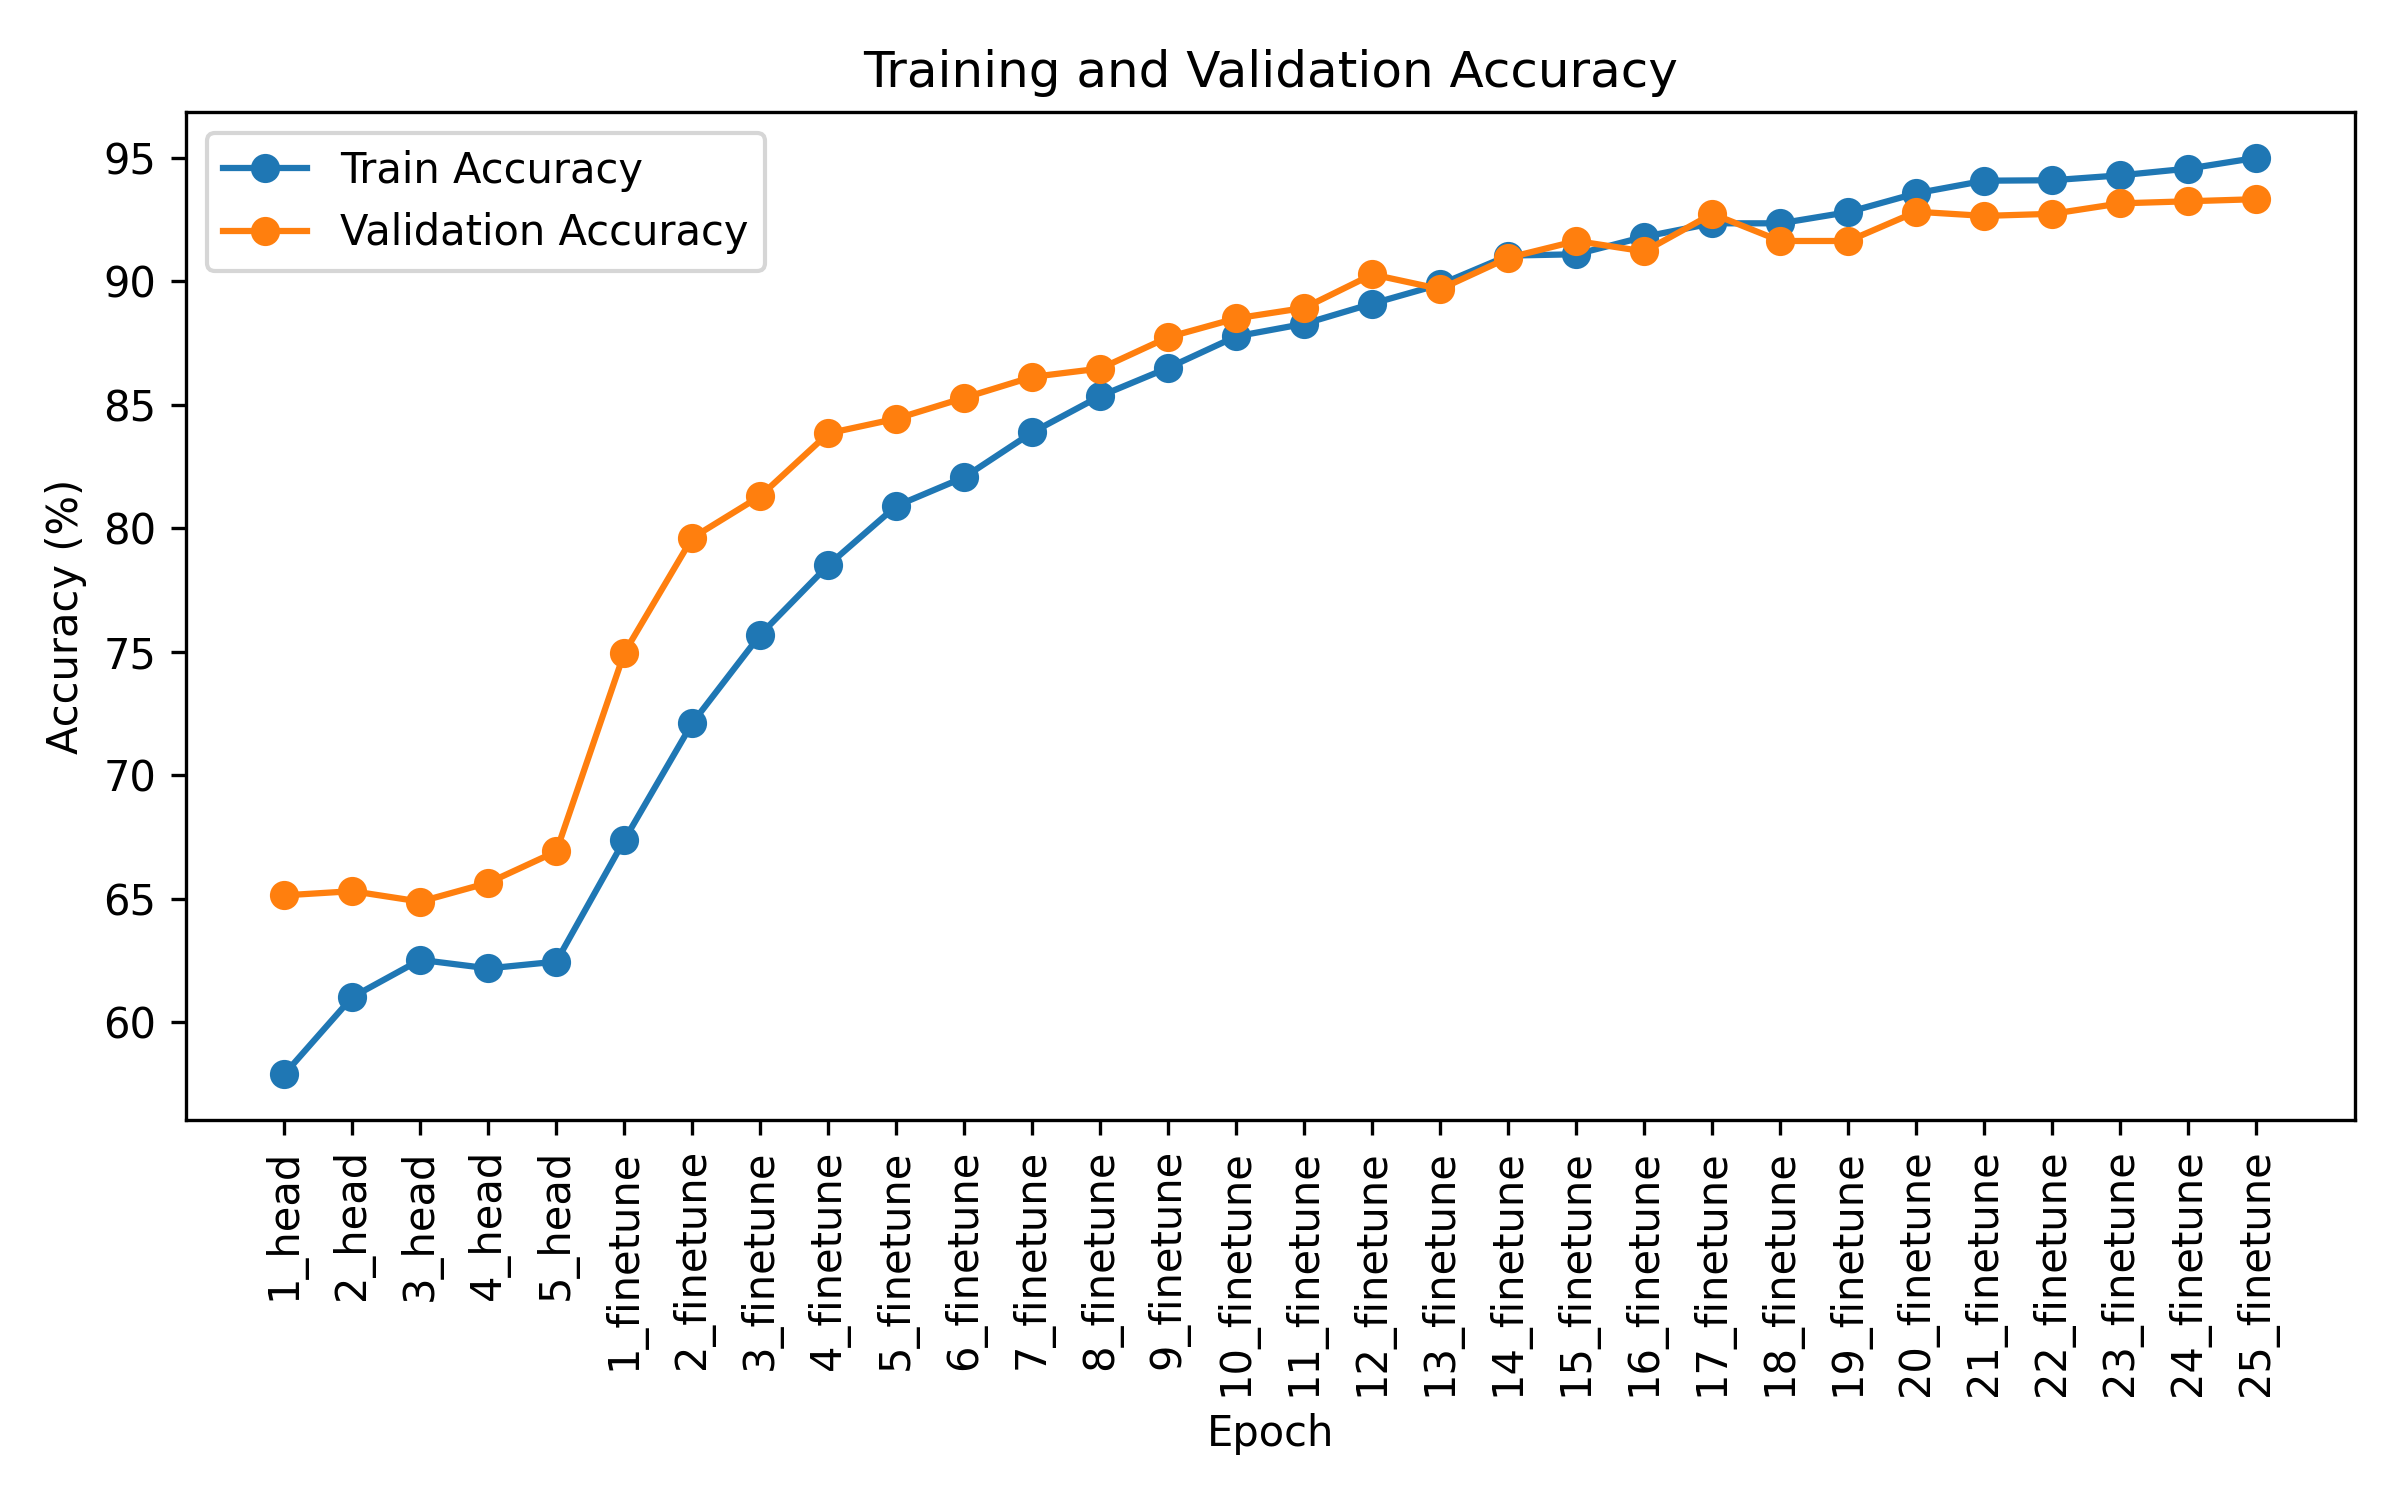
\includegraphics[width=\linewidth]{sec/images/rgb_training_validation_accuracy.png}
\caption{Training and validation accuracy across the warm-up (head) and
fine-tuning epochs on the leakage-aware split. The gradual climb, rather than an
instant jump, indicates genuine learning rather than leakage.}
\label{fig:curves}
\end{figure}

\begin{figure}[t]
\centering
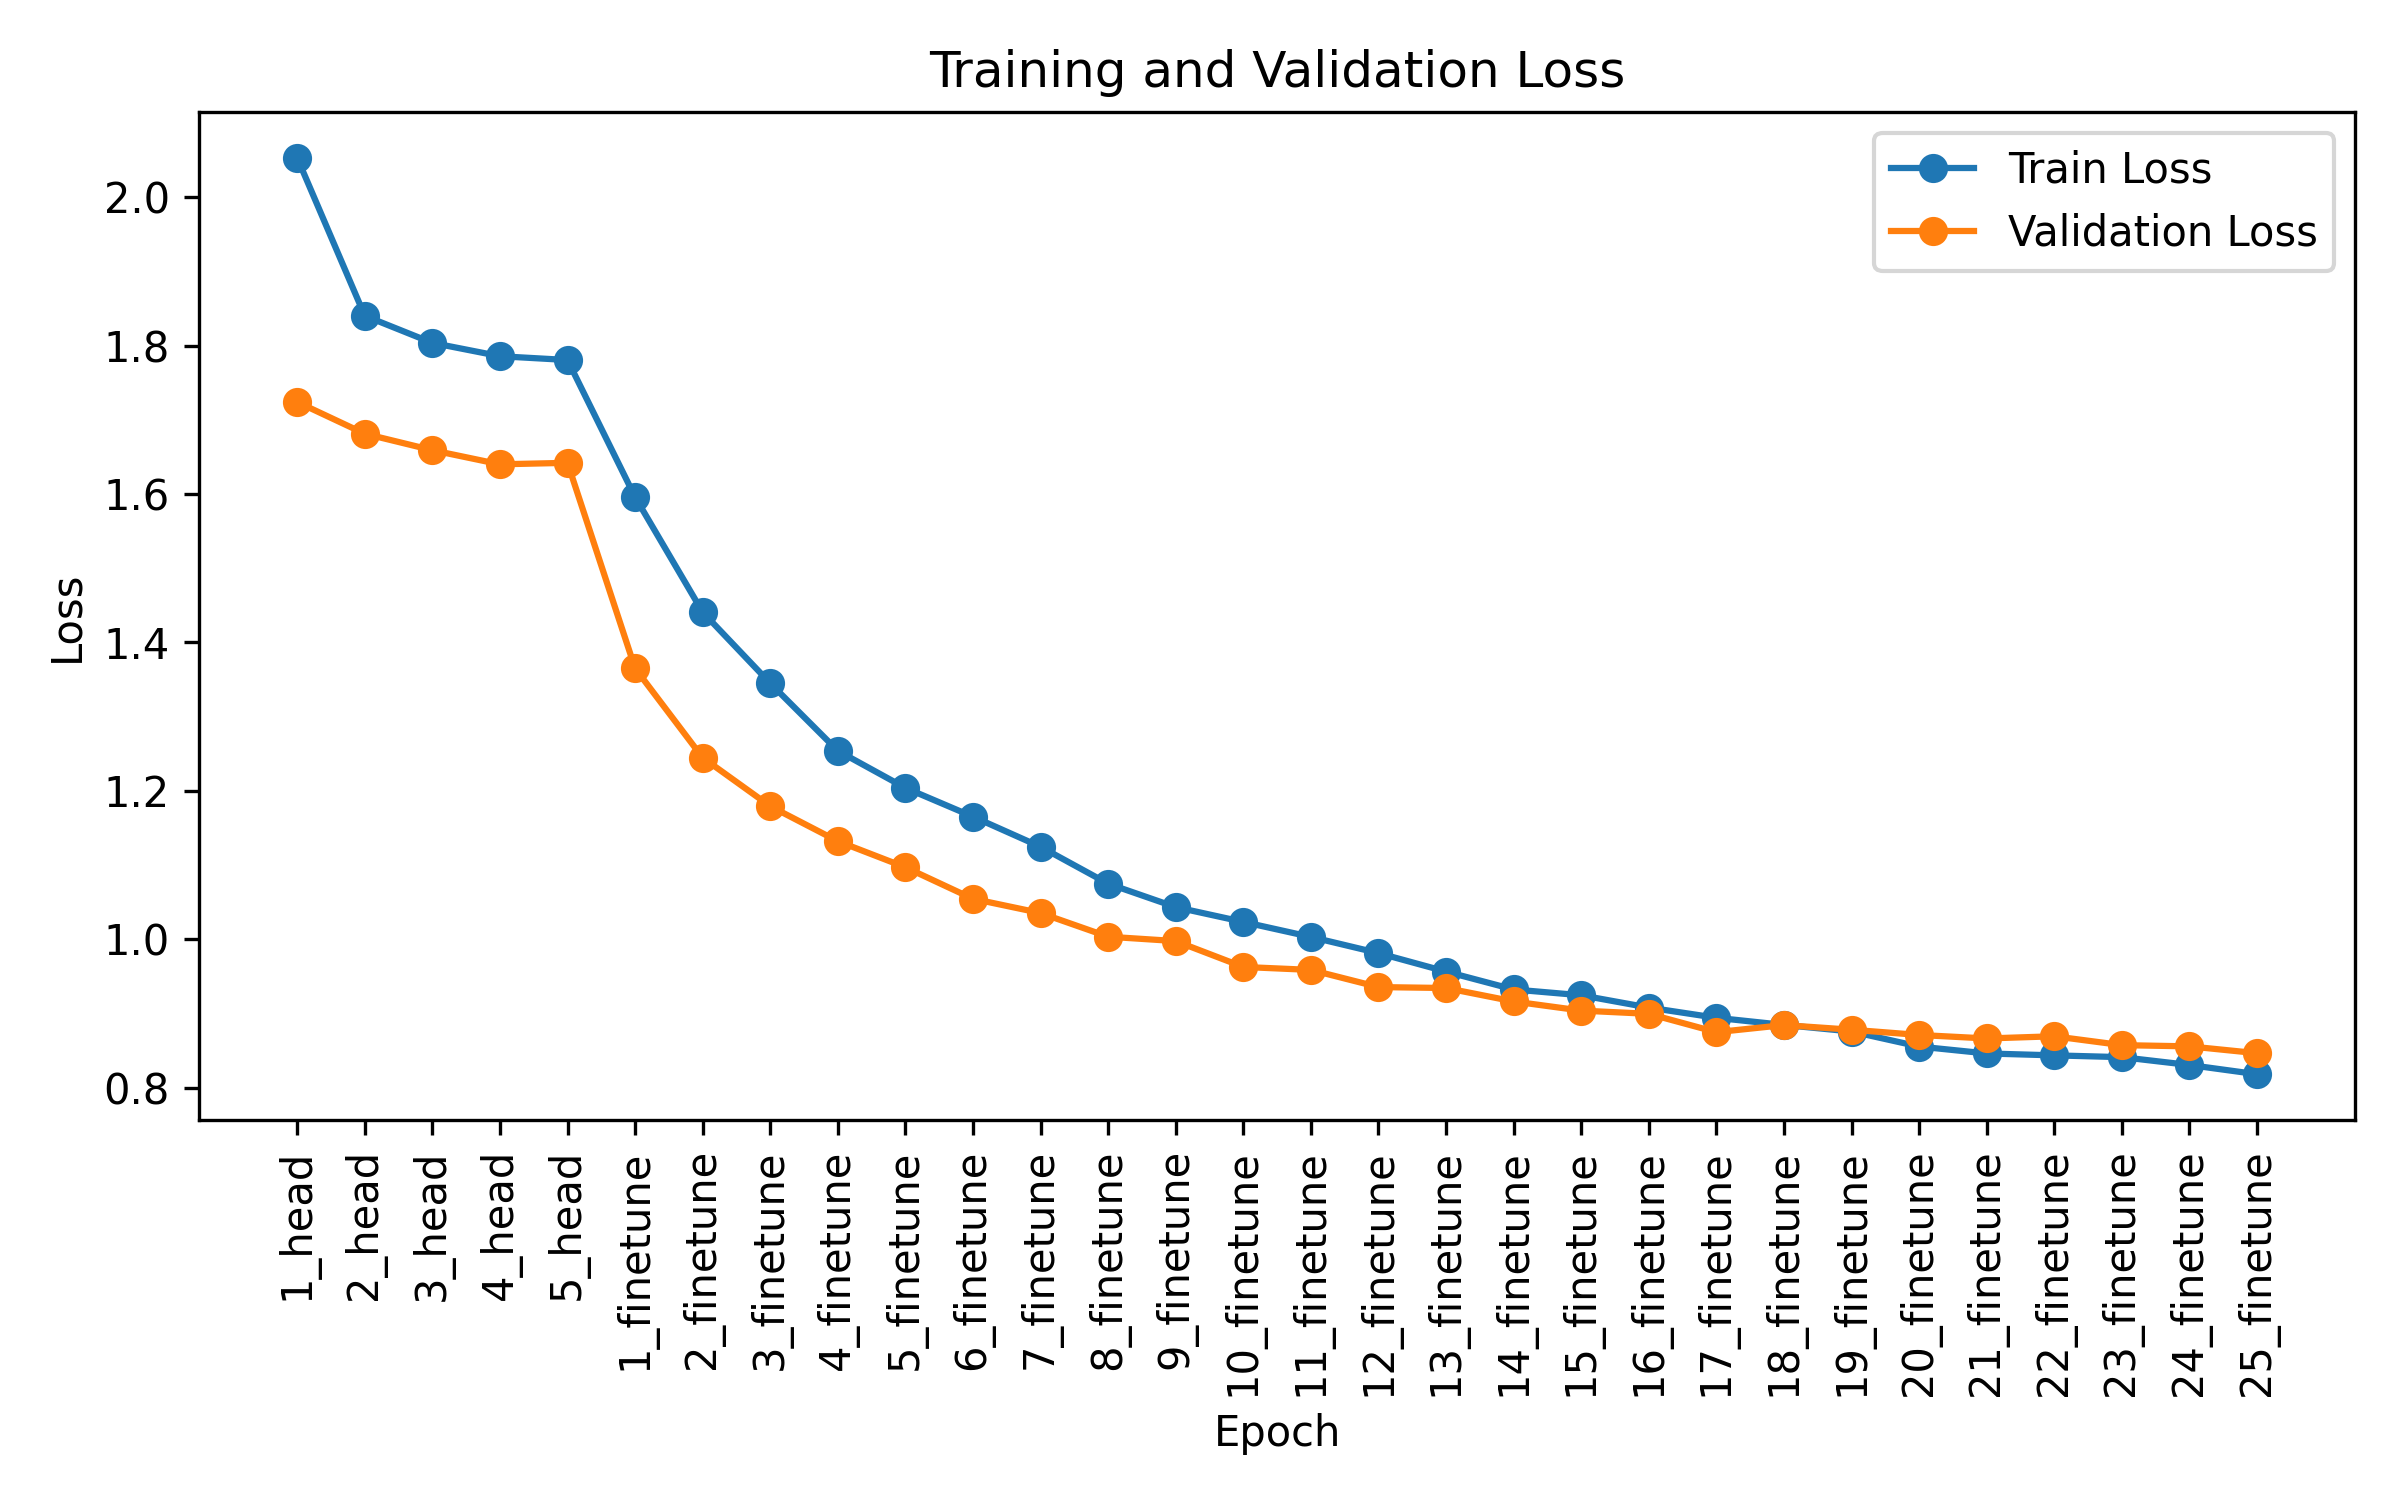
\includegraphics[width=\linewidth]{sec/images/rgb_training_validation_loss.png}
\caption{Training and validation loss over the same epochs. Both decrease smoothly;
label smoothing keeps the loss from reaching zero.}
\label{fig:loss}
\end{figure}

\subsection{Evaluation Across Regimes: The Data Leakage Analysis}
Our first model reached 99.26\% test accuracy, but this number came from a random
image-level split and is inflated by leakage. To make this concrete, we compare
three very different evaluation settings in Table~\ref{tab:regimes}.

\begin{table}[t]
\centering
\caption{Accuracy under different evaluation settings. The sanity check only
confirms that the inference pipeline is correct; it is not a generalization
measure.}
\label{tab:regimes}
\begin{tabular}{lll c}
\toprule
\textbf{Setting} & \textbf{Split} & \textbf{Test set} & \textbf{Acc.}\\
\midrule
Original model      & Random (image) & ArASL          & 99.26\% \\
Sanity check        & ---            & ArASL          & 98.75\% \\
Cross-dataset       & Train on ArASL & RGB (31 cls.)  & 48.78\% \\
\textbf{Clean retrain} & \textbf{Cluster-based} & \textbf{Held-out} & \textbf{94.33\%} \\
\bottomrule
\end{tabular}
\end{table}

We first ran a sanity check: using the exact inference pipeline, the original model
scored 98.75\% on a small ArASL sample. This only tells us the pipeline (model
loading, class order, preprocessing) is correct, not that the model generalizes.

The real test is the cross-dataset evaluation. When we ran the ArASL-trained model
on the independent RGB dataset, accuracy dropped to 48.78\%. That is still well
above random chance (about 3\% for 31 classes), so the model did learn real
features, but it is far from the 99.26\% it reported on its own dataset. Looking at
the per-class scores, the pair \texttt{ta}/\texttt{taa} scored zero, which points
to a label-matching or sign-convention mismatch for that pair rather than a model
failure; setting it aside raises the figure to about 52\%.

The drop from 99.26\% to 48.78\% should not be blamed entirely on leakage. It mixes
three things: real data leakage, a domain shift (different people, lighting,
cameras, and backgrounds), and the class mismatch above. Retraining with the
leakage-aware split removes the leakage part and gives the honest 94.33\% reported
in Table~\ref{tab:regimes}.

\subsection{Quantitative Results}
Table~\ref{tab:results} summarizes the final model. After retraining on the color
data with the clean split, the model reaches 94.33\% on a held-out test set, with a
weighted F1-score of 94.36\%. This is the accuracy we report as a fair estimate of
its real performance.

\begin{table}[t]
\centering
\caption{Final results of the leakage-aware ArSignTutor model on the clean
held-out test set.}
\label{tab:results}
\begin{tabular}{ll}
\toprule
\textbf{Metric} & \textbf{Value}\\
\midrule
Test Accuracy        & 94.33\% \\
Validation Accuracy  & 93.32\% \\
Precision (weighted) & 94.59\% \\
Recall (weighted)    & 94.33\% \\
F1-score (weighted)  & 94.36\% \\
Cross-dataset (prior model) & 48.78\% \\
Number of Classes    & 31 \\
Architecture         & MobileNetV2 \\
Input Resolution     & $224 \times 224$ \\
Optimizer            & AdamW \\
\bottomrule
\end{tabular}
\end{table}

Figure~\ref{fig:confusion} shows the confusion matrix on the clean test set. Most
of the weight is on the diagonal, and the errors that remain fall between letters
with very similar hand shapes, which is the natural limit of recognizing a single
still image. Table~\ref{tab:perclass} breaks the accuracy down by class. Every class
reaches an F1-score above 0.85, and no class collapses, which shows the model
learned all 31 letters rather than trading some off against others.

\begin{figure*}[t]
\centering

\includegraphics[width=0.8\linewidth]{sec/images/clean_rgb_confusion_matrix.png}
\caption{Confusion matrix on the clean held-out test set. The strong diagonal shows
correct classification across the 31 classes; the few off-diagonal errors fall
between letters with similar hand shapes (e.g., \texttt{dal} and \texttt{thal},
which differ only by a dot).}
\label{fig:confusion}
\end{figure*}

\begin{figure*}[t]
\centering
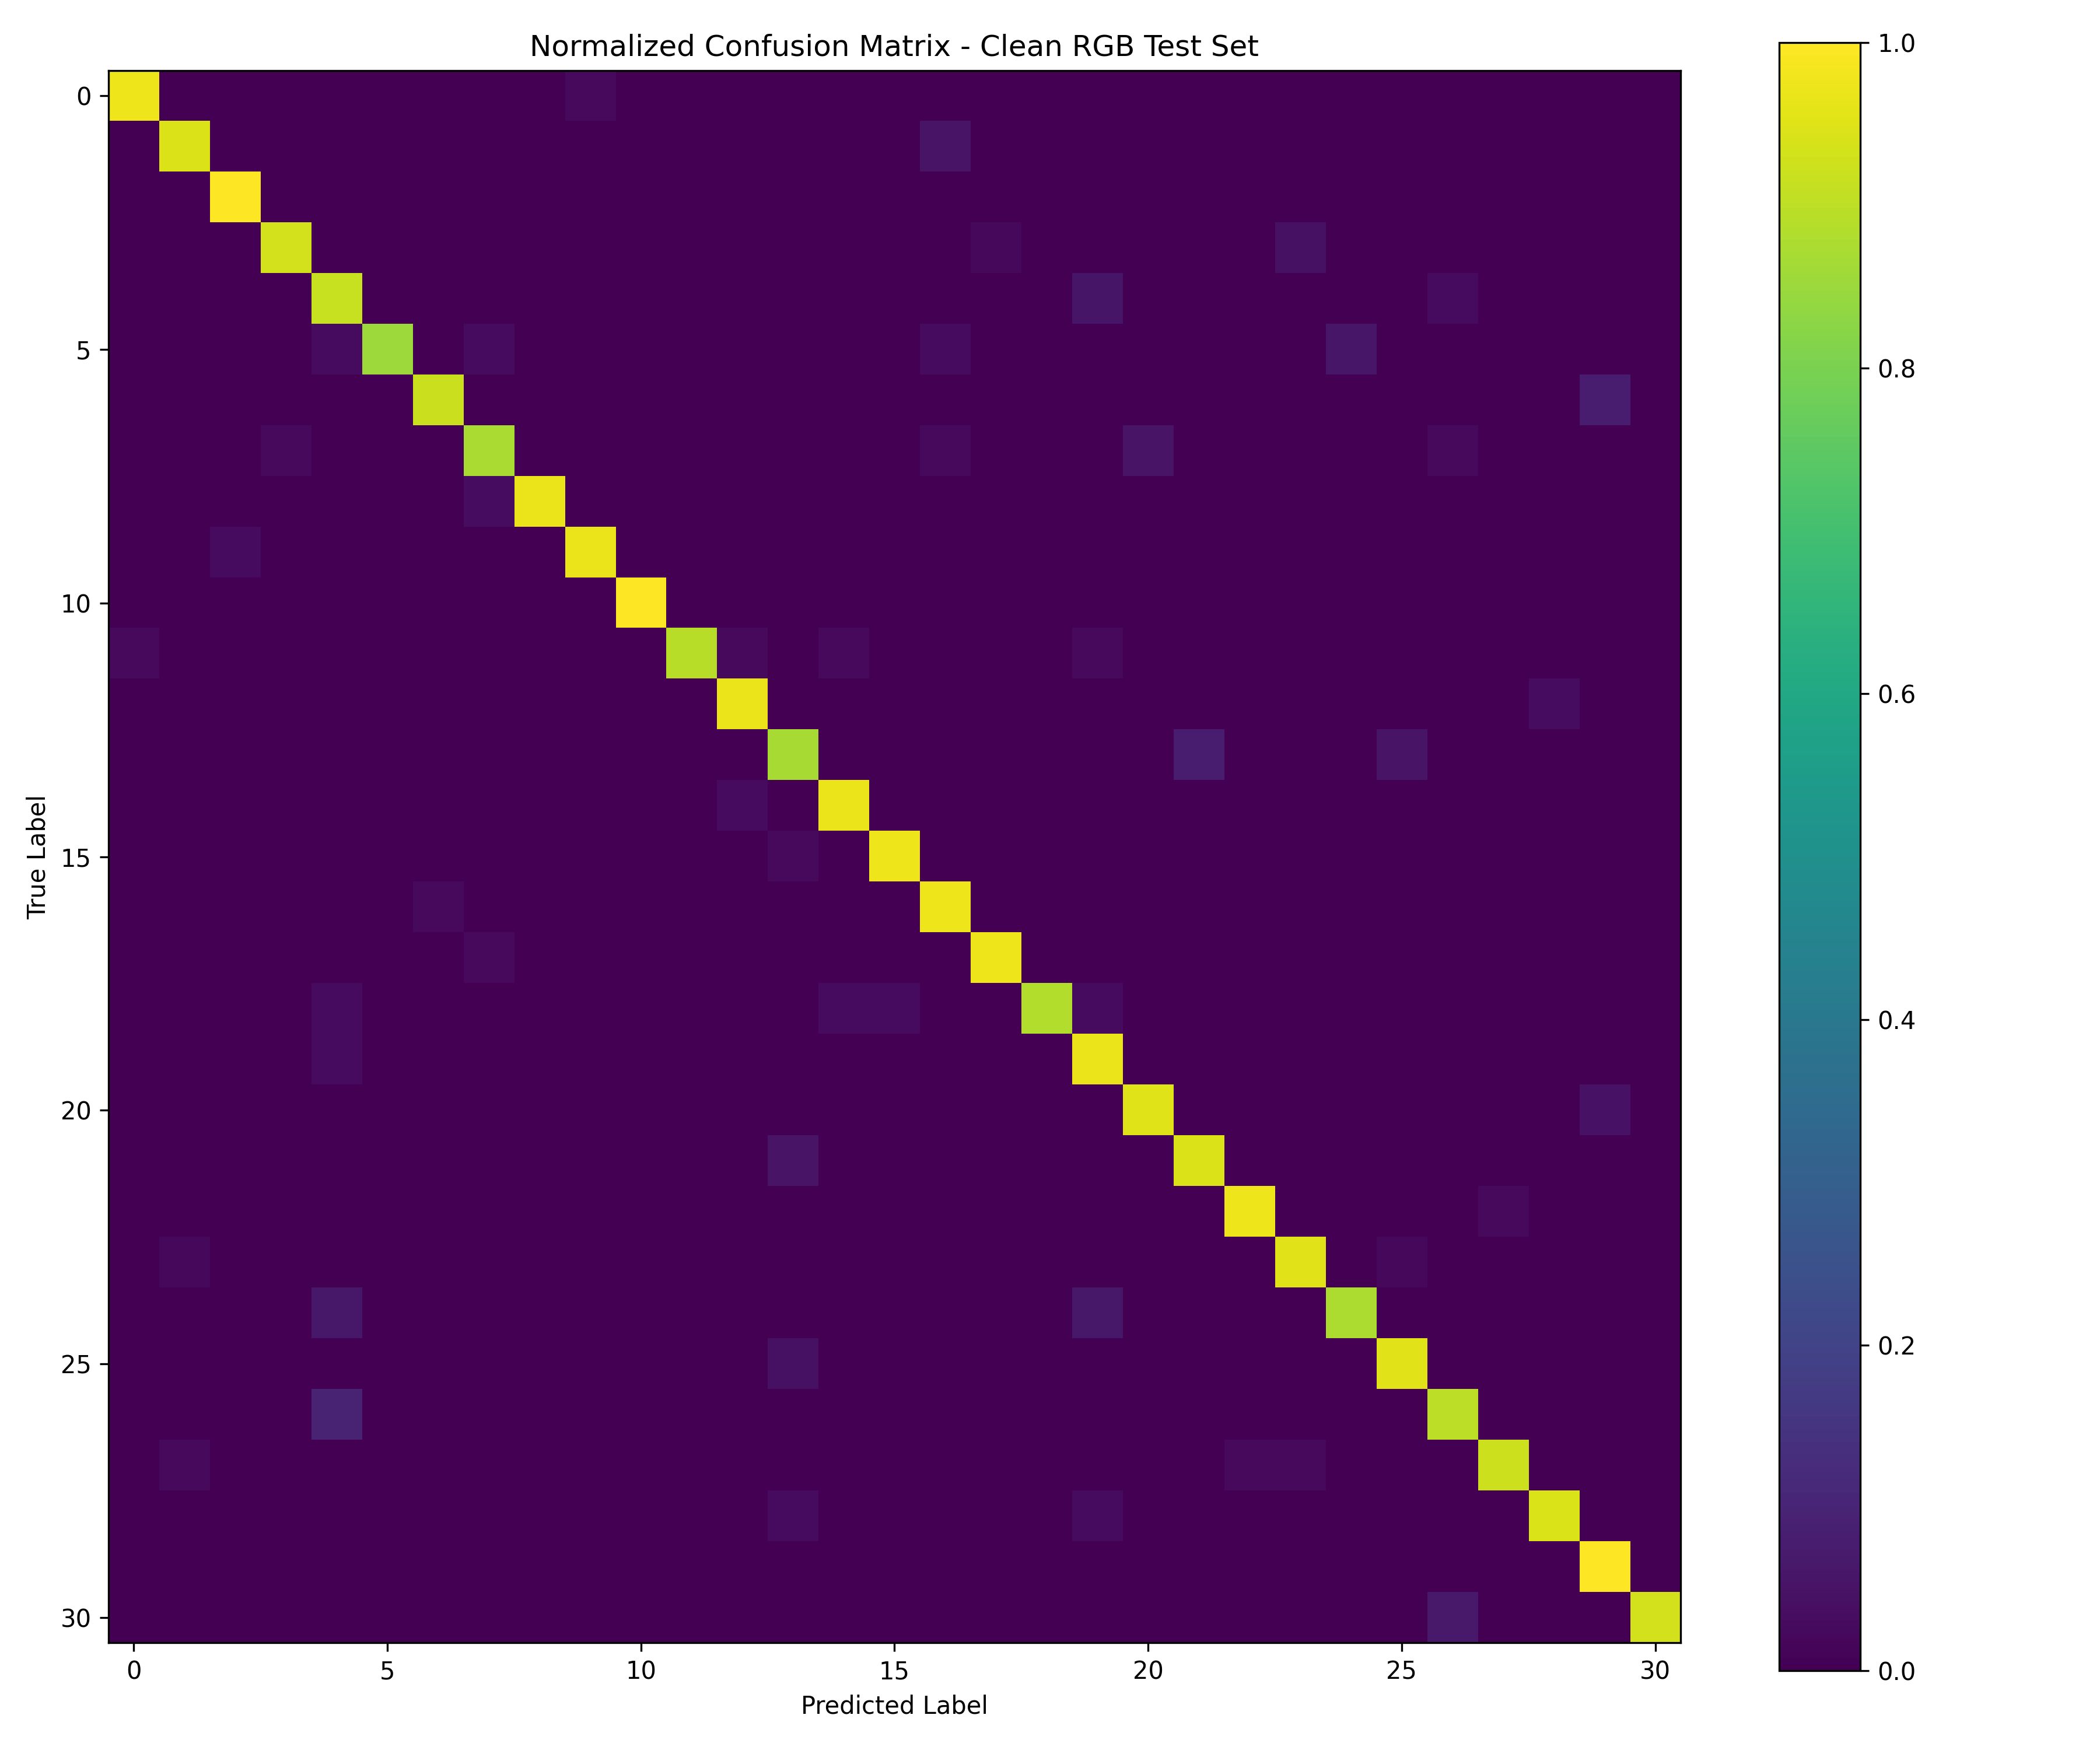
\includegraphics[width=0.8\linewidth]{sec/images/clean_rgb_confusion_matrix_normalized.png}
\caption{Normalized confusion matrix showing class-wise recognition performance on the clean RGB test set.}
\label{fig:confusion-normalized}
\end{figure*}

\begin{table}[t]
\centering
\caption{Per-class precision, recall, and F1-score on the clean test set.}
\label{tab:perclass}
\small
\begin{tabular}{lccc}
\toprule
\textbf{Class} & \textbf{Precision} & \textbf{Recall} & \textbf{F1} \\
\midrule
ain   & 0.97 & 0.97 & 0.97 \\
al    & 0.95 & 0.95 & 0.95 \\
aleff & 0.98 & 1.00 & 0.99 \\
bb    & 0.98 & 0.93 & 0.95 \\
dal   & 0.80 & 0.91 & 0.85 \\
dha   & 1.00 & 0.85 & 0.92 \\
dhad  & 0.97 & 0.92 & 0.95 \\
fa    & 0.92 & 0.87 & 0.89 \\
gaaf  & 1.00 & 0.97 & 0.98 \\
ghain & 0.97 & 0.97 & 0.97 \\
ha    & 1.00 & 1.00 & 1.00 \\
haa   & 1.00 & 0.89 & 0.94 \\
jeem  & 0.94 & 0.97 & 0.95 \\
kaaf  & 0.85 & 0.87 & 0.86 \\
khaa  & 0.95 & 0.97 & 0.96 \\
la    & 0.98 & 0.98 & 0.98 \\
laam  & 0.90 & 0.97 & 0.94 \\
meem  & 0.97 & 0.97 & 0.97 \\
nun   & 1.00 & 0.89 & 0.94 \\
ra    & 0.83 & 0.97 & 0.90 \\
saad  & 0.95 & 0.95 & 0.95 \\
seen  & 0.93 & 0.95 & 0.94 \\
sheen & 0.98 & 0.98 & 0.98 \\
ta    & 0.94 & 0.96 & 0.95 \\
taa   & 0.93 & 0.88 & 0.90 \\
thaa  & 0.94 & 0.96 & 0.95 \\
thal  & 0.87 & 0.90 & 0.89 \\
toot  & 0.97 & 0.93 & 0.95 \\
waw   & 0.97 & 0.94 & 0.96 \\
ya    & 0.90 & 1.00 & 0.95 \\
zay   & 1.00 & 0.93 & 0.96 \\
\midrule
\textbf{Weighted avg} & \textbf{0.95} & \textbf{0.94} & \textbf{0.94} \\
\bottomrule
\end{tabular}
\end{table}

\subsection{Analysis of Generalization Performance}

One of the most important findings of this work is the difference between benchmark accuracy and true generalization performance. The initial MobileNetV2 model achieved more than 99% accuracy on the original ArASL dataset. However, when evaluated on an independent RGB Arabic Sign Language dataset, performance dropped to 48.78%.

This result highlights the importance of evaluating sign language recognition systems under realistic conditions. High performance on a single dataset does not necessarily guarantee strong generalization to new users, different cameras, lighting conditions, or collection environments.

After applying the leakage-aware cluster-based splitting strategy and performing domain adaptation on the RGB dataset, the final model achieved 94.33% test accuracy. This substantial improvement demonstrates that the model successfully adapted to the target domain while maintaining strong generalization capability.

These findings suggest that careful dataset design and evaluation protocols are as important as model architecture when developing practical sign language recognition systems.

\subsection{Analysis of Generalization Performance}

One of the most important findings of this work is the difference between benchmark accuracy and true generalization performance...

...
\subsection{Real-Time System Evaluation}
We put the trained model into a real-time webcam app built with Streamlit and
OpenCV. The user signs a letter in front of the camera and gets an immediate
prediction. To help the model focus on the gesture, we crop to the hand region
before classifying, which cuts down on background distractions. In testing, the
system worked well under normal conditions, though accuracy still depends on
lighting, hand position, camera quality, and how similar two letters look.

On top of single-letter prediction, the app includes a spelling tutor that walks
the user through Arabic words one letter at a time. This turns the project from a
plain classifier into something a learner can actually practice with.